\begin{figure}
\centering
\begingroup
\renewcommand{\arraystretch}{1.7}
\begin{tabular}{rc@{}c@{}c@{}c@{}c@{}c@{}c@{}c@{}c@{}c@{}c@{}c@{}c@{}c@{}c@{}c@{}c@{}c@{}c@{}c@{}}
$G(\z)\phantom{)}$ &

\includegraphics[width=0.037\linewidth,valign=c]{figs/mnist_bigan_samples/sample_0_0.png} &

\includegraphics[width=0.037\linewidth,valign=c]{figs/mnist_bigan_samples/sample_1_0.png} &

\includegraphics[width=0.037\linewidth,valign=c]{figs/mnist_bigan_samples/sample_2_0.png} &

\includegraphics[width=0.037\linewidth,valign=c]{figs/mnist_bigan_samples/sample_3_0.png} &

\includegraphics[width=0.037\linewidth,valign=c]{figs/mnist_bigan_samples/sample_4_0.png} &

\includegraphics[width=0.037\linewidth,valign=c]{figs/mnist_bigan_samples/sample_5_0.png} &

\includegraphics[width=0.037\linewidth,valign=c]{figs/mnist_bigan_samples/sample_6_0.png} &

\includegraphics[width=0.037\linewidth,valign=c]{figs/mnist_bigan_samples/sample_7_0.png} &

\includegraphics[width=0.037\linewidth,valign=c]{figs/mnist_bigan_samples/sample_8_0.png} &

\includegraphics[width=0.037\linewidth,valign=c]{figs/mnist_bigan_samples/sample_9_0.png} &

\includegraphics[width=0.037\linewidth,valign=c]{figs/mnist_bigan_samples/sample_0_1.png} &

\includegraphics[width=0.037\linewidth,valign=c]{figs/mnist_bigan_samples/sample_1_1.png} &

\includegraphics[width=0.037\linewidth,valign=c]{figs/mnist_bigan_samples/sample_2_1.png} &

\includegraphics[width=0.037\linewidth,valign=c]{figs/mnist_bigan_samples/sample_3_1.png} &

\includegraphics[width=0.037\linewidth,valign=c]{figs/mnist_bigan_samples/sample_4_1.png} &

\includegraphics[width=0.037\linewidth,valign=c]{figs/mnist_bigan_samples/sample_5_1.png} &

\includegraphics[width=0.037\linewidth,valign=c]{figs/mnist_bigan_samples/sample_6_1.png} &

\includegraphics[width=0.037\linewidth,valign=c]{figs/mnist_bigan_samples/sample_7_1.png} &

\includegraphics[width=0.037\linewidth,valign=c]{figs/mnist_bigan_samples/sample_8_1.png} &

\includegraphics[width=0.037\linewidth,valign=c]{figs/mnist_bigan_samples/sample_9_1.png} \\
\midrule
$\x\phantom{))}$ &

\includegraphics[width=0.037\linewidth,valign=c]{figs/mnist_real/sample_0_0.png} &

\includegraphics[width=0.037\linewidth,valign=c]{figs/mnist_real/sample_1_0.png} &

\includegraphics[width=0.037\linewidth,valign=c]{figs/mnist_real/sample_2_0.png} &

\includegraphics[width=0.037\linewidth,valign=c]{figs/mnist_real/sample_3_0.png} &

\includegraphics[width=0.037\linewidth,valign=c]{figs/mnist_real/sample_4_0.png} &

\includegraphics[width=0.037\linewidth,valign=c]{figs/mnist_real/sample_5_0.png} &

\includegraphics[width=0.037\linewidth,valign=c]{figs/mnist_real/sample_6_0.png} &

\includegraphics[width=0.037\linewidth,valign=c]{figs/mnist_real/sample_7_0.png} &

\includegraphics[width=0.037\linewidth,valign=c]{figs/mnist_real/sample_8_0.png} &

\includegraphics[width=0.037\linewidth,valign=c]{figs/mnist_real/sample_9_0.png} &

\includegraphics[width=0.037\linewidth,valign=c]{figs/mnist_real/sample_0_1.png} &

\includegraphics[width=0.037\linewidth,valign=c]{figs/mnist_real/sample_1_1.png} &

\includegraphics[width=0.037\linewidth,valign=c]{figs/mnist_real/sample_2_1.png} &

\includegraphics[width=0.037\linewidth,valign=c]{figs/mnist_real/sample_3_1.png} &

\includegraphics[width=0.037\linewidth,valign=c]{figs/mnist_real/sample_4_1.png} &

\includegraphics[width=0.037\linewidth,valign=c]{figs/mnist_real/sample_5_1.png} &

\includegraphics[width=0.037\linewidth,valign=c]{figs/mnist_real/sample_6_1.png} &

\includegraphics[width=0.037\linewidth,valign=c]{figs/mnist_real/sample_7_1.png} &

\includegraphics[width=0.037\linewidth,valign=c]{figs/mnist_real/sample_8_1.png} &
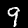
\includegraphics[width=0.037\linewidth,valign=c]{figs/mnist_real/sample_9_1.png} \\
$G(E(\x))$ &

\includegraphics[width=0.037\linewidth,valign=c]{figs/mnist_bigan_regen/sample_0_0.png} &

\includegraphics[width=0.037\linewidth,valign=c]{figs/mnist_bigan_regen/sample_1_0.png} &

\includegraphics[width=0.037\linewidth,valign=c]{figs/mnist_bigan_regen/sample_2_0.png} &

\includegraphics[width=0.037\linewidth,valign=c]{figs/mnist_bigan_regen/sample_3_0.png} &

\includegraphics[width=0.037\linewidth,valign=c]{figs/mnist_bigan_regen/sample_4_0.png} &

\includegraphics[width=0.037\linewidth,valign=c]{figs/mnist_bigan_regen/sample_5_0.png} &

\includegraphics[width=0.037\linewidth,valign=c]{figs/mnist_bigan_regen/sample_6_0.png} &

\includegraphics[width=0.037\linewidth,valign=c]{figs/mnist_bigan_regen/sample_7_0.png} &

\includegraphics[width=0.037\linewidth,valign=c]{figs/mnist_bigan_regen/sample_8_0.png} &

\includegraphics[width=0.037\linewidth,valign=c]{figs/mnist_bigan_regen/sample_9_0.png} &

\includegraphics[width=0.037\linewidth,valign=c]{figs/mnist_bigan_regen/sample_0_1.png} &

\includegraphics[width=0.037\linewidth,valign=c]{figs/mnist_bigan_regen/sample_1_1.png} &

\includegraphics[width=0.037\linewidth,valign=c]{figs/mnist_bigan_regen/sample_2_1.png} &

\includegraphics[width=0.037\linewidth,valign=c]{figs/mnist_bigan_regen/sample_3_1.png} &

\includegraphics[width=0.037\linewidth,valign=c]{figs/mnist_bigan_regen/sample_4_1.png} &

\includegraphics[width=0.037\linewidth,valign=c]{figs/mnist_bigan_regen/sample_5_1.png} &

\includegraphics[width=0.037\linewidth,valign=c]{figs/mnist_bigan_regen/sample_6_1.png} &

\includegraphics[width=0.037\linewidth,valign=c]{figs/mnist_bigan_regen/sample_7_1.png} &

\includegraphics[width=0.037\linewidth,valign=c]{figs/mnist_bigan_regen/sample_8_1.png} &

\includegraphics[width=0.037\linewidth,valign=c]{figs/mnist_bigan_regen/sample_9_1.png} \\
\end{tabular}
\endgroup
\caption{
Qualitative results for permutation-invariant MNIST BiGAN training,
including generator samples $G(\z)$,
real data $\x$,
and corresponding reconstructions $G(E(\x))$.
}
\lblfig{mnistqual}
\end{figure}
